% Created by tikzDevice version 0.12 on 2019-04-30 20:46:52
% !TEX encoding = UTF-8 Unicode
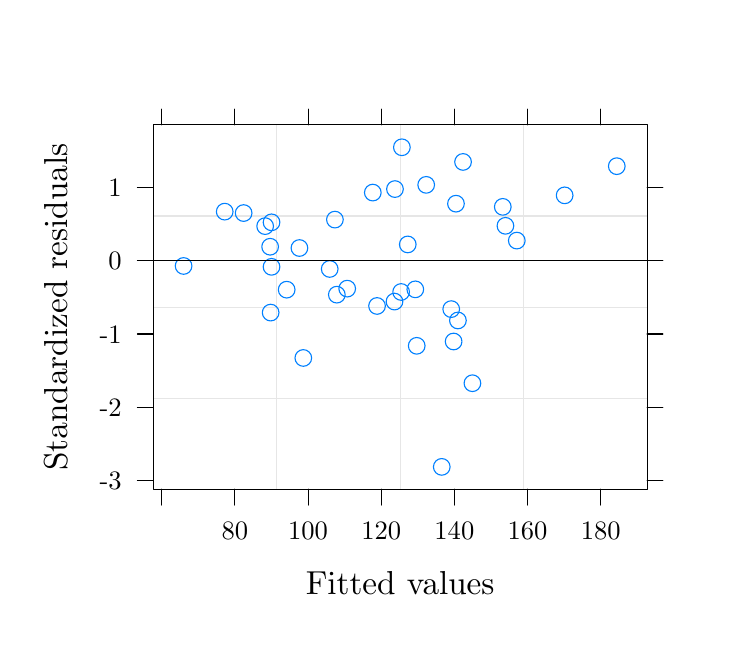
\begin{tikzpicture}[x=1pt,y=1pt]
\definecolor{fillColor}{RGB}{255,255,255}
\path[use as bounding box,fill=fillColor,fill opacity=0.00] (0,0) rectangle (252.94,216.81);
\begin{scope}
\path[clip] (  0.00,  0.00) rectangle (252.94,216.81);

\path[] (  0.00,  0.00) rectangle (252.94,216.81);
\definecolor{drawColor}{RGB}{0,0,0}

\node[text=drawColor,anchor=base,inner sep=0pt, outer sep=0pt, scale=  1.20] at (134.60, 12.05) {Fitted values};
\end{scope}
\begin{scope}
\path[clip] (  0.00,  0.00) rectangle (252.94,216.81);
\definecolor{drawColor}{RGB}{0,0,0}

\node[text=drawColor,rotate= 90.00,anchor=base,inner sep=0pt, outer sep=0pt, scale=  1.20] at ( 14.29,115.84) {Standardized residuals};
\end{scope}
\begin{scope}
\path[clip] (  0.00,  0.00) rectangle (252.94,216.81);
\definecolor{drawColor}{RGB}{0,0,0}

\path[draw=drawColor,line width= 0.4pt,line join=round,line cap=round] ( 48.45,181.67) -- ( 48.45,187.36);

\path[draw=drawColor,line width= 0.4pt,line join=round,line cap=round] ( 74.89,181.67) -- ( 74.89,187.36);

\path[draw=drawColor,line width= 0.4pt,line join=round,line cap=round] (101.32,181.67) -- (101.32,187.36);

\path[draw=drawColor,line width= 0.4pt,line join=round,line cap=round] (127.76,181.67) -- (127.76,187.36);

\path[draw=drawColor,line width= 0.4pt,line join=round,line cap=round] (154.19,181.67) -- (154.19,187.36);

\path[draw=drawColor,line width= 0.4pt,line join=round,line cap=round] (180.63,181.67) -- (180.63,187.36);

\path[draw=drawColor,line width= 0.4pt,line join=round,line cap=round] (207.06,181.67) -- (207.06,187.36);
\end{scope}
\begin{scope}
\path[clip] (  0.00,  0.00) rectangle (252.94,216.81);
\definecolor{drawColor}{RGB}{0,0,0}

\path[draw=drawColor,line width= 0.4pt,line join=round,line cap=round] ( 45.38, 53.19) -- ( 39.69, 53.19);

\path[draw=drawColor,line width= 0.4pt,line join=round,line cap=round] ( 45.38, 79.66) -- ( 39.69, 79.66);

\path[draw=drawColor,line width= 0.4pt,line join=round,line cap=round] ( 45.38,106.12) -- ( 39.69,106.12);

\path[draw=drawColor,line width= 0.4pt,line join=round,line cap=round] ( 45.38,132.59) -- ( 39.69,132.59);

\path[draw=drawColor,line width= 0.4pt,line join=round,line cap=round] ( 45.38,159.06) -- ( 39.69,159.06);

\node[text=drawColor,anchor=base east,inner sep=0pt, outer sep=0pt, scale=  0.96] at ( 34.00, 49.88) {-3};

\node[text=drawColor,anchor=base east,inner sep=0pt, outer sep=0pt, scale=  0.96] at ( 34.00, 76.35) {-2};

\node[text=drawColor,anchor=base east,inner sep=0pt, outer sep=0pt, scale=  0.96] at ( 34.00,102.82) {-1};

\node[text=drawColor,anchor=base east,inner sep=0pt, outer sep=0pt, scale=  0.96] at ( 34.00,129.28) {0};

\node[text=drawColor,anchor=base east,inner sep=0pt, outer sep=0pt, scale=  0.96] at ( 34.00,155.75) {1};
\end{scope}
\begin{scope}
\path[clip] (  0.00,  0.00) rectangle (252.94,216.81);
\definecolor{drawColor}{RGB}{0,0,0}

\path[draw=drawColor,line width= 0.4pt,line join=round,line cap=round] ( 48.45, 50.02) -- ( 48.45, 44.32);

\path[draw=drawColor,line width= 0.4pt,line join=round,line cap=round] ( 74.89, 50.02) -- ( 74.89, 44.32);

\path[draw=drawColor,line width= 0.4pt,line join=round,line cap=round] (101.32, 50.02) -- (101.32, 44.32);

\path[draw=drawColor,line width= 0.4pt,line join=round,line cap=round] (127.76, 50.02) -- (127.76, 44.32);

\path[draw=drawColor,line width= 0.4pt,line join=round,line cap=round] (154.19, 50.02) -- (154.19, 44.32);

\path[draw=drawColor,line width= 0.4pt,line join=round,line cap=round] (180.63, 50.02) -- (180.63, 44.32);

\path[draw=drawColor,line width= 0.4pt,line join=round,line cap=round] (207.06, 50.02) -- (207.06, 44.32);

\node[text=drawColor,anchor=base,inner sep=0pt, outer sep=0pt, scale=  0.96] at ( 74.89, 32.02) {80};

\node[text=drawColor,anchor=base,inner sep=0pt, outer sep=0pt, scale=  0.96] at (101.32, 32.02) {100};

\node[text=drawColor,anchor=base,inner sep=0pt, outer sep=0pt, scale=  0.96] at (127.76, 32.02) {120};

\node[text=drawColor,anchor=base,inner sep=0pt, outer sep=0pt, scale=  0.96] at (154.19, 32.02) {140};

\node[text=drawColor,anchor=base,inner sep=0pt, outer sep=0pt, scale=  0.96] at (180.63, 32.02) {160};

\node[text=drawColor,anchor=base,inner sep=0pt, outer sep=0pt, scale=  0.96] at (207.06, 32.02) {180};

\path[draw=drawColor,line width= 0.4pt,line join=round,line cap=round] (223.83, 53.19) -- (229.52, 53.19);

\path[draw=drawColor,line width= 0.4pt,line join=round,line cap=round] (223.83, 79.66) -- (229.52, 79.66);

\path[draw=drawColor,line width= 0.4pt,line join=round,line cap=round] (223.83,106.12) -- (229.52,106.12);

\path[draw=drawColor,line width= 0.4pt,line join=round,line cap=round] (223.83,132.59) -- (229.52,132.59);

\path[draw=drawColor,line width= 0.4pt,line join=round,line cap=round] (223.83,159.06) -- (229.52,159.06);
\end{scope}
\begin{scope}
\path[clip] ( 45.38, 50.02) rectangle (223.83,181.67);
\definecolor{drawColor}{RGB}{230,230,230}

\path[draw=drawColor,line width= 0.4pt,line join=round,line cap=round] ( 45.38, 82.93) -- (223.83, 82.93);

\path[draw=drawColor,line width= 0.4pt,line join=round,line cap=round] ( 45.38,115.84) -- (223.83,115.84);

\path[draw=drawColor,line width= 0.4pt,line join=round,line cap=round] ( 45.38,148.76) -- (223.83,148.76);

\path[draw=drawColor,line width= 0.4pt,line join=round,line cap=round] ( 89.99, 50.02) -- ( 89.99,181.67);

\path[draw=drawColor,line width= 0.4pt,line join=round,line cap=round] (134.60, 50.02) -- (134.60,181.67);

\path[draw=drawColor,line width= 0.4pt,line join=round,line cap=round] (179.22, 50.02) -- (179.22,181.67);
\definecolor{drawColor}{RGB}{0,128,255}

\path[draw=drawColor,line width= 0.4pt,line join=round,line cap=round] (171.68,152.06) circle (  3.01);

\path[draw=drawColor,line width= 0.4pt,line join=round,line cap=round] ( 85.81,145.10) circle (  3.01);

\path[draw=drawColor,line width= 0.4pt,line join=round,line cap=round] ( 99.60, 97.46) circle (  3.01);

\path[draw=drawColor,line width= 0.4pt,line join=round,line cap=round] (194.03,156.22) circle (  3.01);

\path[draw=drawColor,line width= 0.4pt,line join=round,line cap=round] (160.71, 88.33) circle (  3.01);

\path[draw=drawColor,line width= 0.4pt,line join=round,line cap=round] (172.64,145.21) circle (  3.01);

\path[draw=drawColor,line width= 0.4pt,line join=round,line cap=round] (135.22,173.59) circle (  3.01);

\path[draw=drawColor,line width= 0.4pt,line join=round,line cap=round] (176.74,139.87) circle (  3.01);

\path[draw=drawColor,line width= 0.4pt,line join=round,line cap=round] ( 87.61,137.65) circle (  3.01);

\path[draw=drawColor,line width= 0.4pt,line join=round,line cap=round] (144.00,160.01) circle (  3.01);

\path[draw=drawColor,line width= 0.4pt,line join=round,line cap=round] ( 56.34,130.70) circle (  3.01);

\path[draw=drawColor,line width= 0.4pt,line join=round,line cap=round] (155.47,111.01) circle (  3.01);

\path[draw=drawColor,line width= 0.4pt,line join=round,line cap=round] (124.71,157.22) circle (  3.01);

\path[draw=drawColor,line width= 0.4pt,line join=round,line cap=round] ( 87.80,113.85) circle (  3.01);

\path[draw=drawColor,line width= 0.4pt,line join=round,line cap=round] (212.87,166.76) circle (  3.01);

\path[draw=drawColor,line width= 0.4pt,line join=round,line cap=round] (126.24,116.25) circle (  3.01);

\path[draw=drawColor,line width= 0.4pt,line join=round,line cap=round] (134.95,121.30) circle (  3.01);

\path[draw=drawColor,line width= 0.4pt,line join=round,line cap=round] (111.71,120.33) circle (  3.01);

\path[draw=drawColor,line width= 0.4pt,line join=round,line cap=round] (132.72,158.49) circle (  3.01);

\path[draw=drawColor,line width= 0.4pt,line join=round,line cap=round] ( 88.12,146.47) circle (  3.01);

\path[draw=drawColor,line width= 0.4pt,line join=round,line cap=round] (137.34,138.48) circle (  3.01);

\path[draw=drawColor,line width= 0.4pt,line join=round,line cap=round] (132.55,117.83) circle (  3.01);

\path[draw=drawColor,line width= 0.4pt,line join=round,line cap=round] ( 98.20,137.19) circle (  3.01);

\path[draw=drawColor,line width= 0.4pt,line join=round,line cap=round] (153.05,115.11) circle (  3.01);

\path[draw=drawColor,line width= 0.4pt,line join=round,line cap=round] (111.02,147.45) circle (  3.01);

\path[draw=drawColor,line width= 0.4pt,line join=round,line cap=round] ( 93.59,122.13) circle (  3.01);

\path[draw=drawColor,line width= 0.4pt,line join=round,line cap=round] ( 78.04,149.82) circle (  3.01);

\path[draw=drawColor,line width= 0.4pt,line join=round,line cap=round] (153.91,103.41) circle (  3.01);

\path[draw=drawColor,line width= 0.4pt,line join=round,line cap=round] (140.58,101.85) circle (  3.01);

\path[draw=drawColor,line width= 0.4pt,line join=round,line cap=round] (140.07,122.25) circle (  3.01);

\path[draw=drawColor,line width= 0.4pt,line join=round,line cap=round] (115.46,122.51) circle (  3.01);

\path[draw=drawColor,line width= 0.4pt,line join=round,line cap=round] ( 88.12,130.39) circle (  3.01);

\path[draw=drawColor,line width= 0.4pt,line join=round,line cap=round] (149.63, 58.10) circle (  3.01);

\path[draw=drawColor,line width= 0.4pt,line join=round,line cap=round] (157.32,168.29) circle (  3.01);

\path[draw=drawColor,line width= 0.4pt,line join=round,line cap=round] (109.14,129.62) circle (  3.01);

\path[draw=drawColor,line width= 0.4pt,line join=round,line cap=round] ( 71.20,150.33) circle (  3.01);

\path[draw=drawColor,line width= 0.4pt,line join=round,line cap=round] (154.76,153.21) circle (  3.01);
\definecolor{drawColor}{RGB}{0,0,0}

\path[draw=drawColor,line width= 0.4pt,line join=round,line cap=round] ( 45.38,132.59) -- (223.83,132.59);
\end{scope}
\begin{scope}
\path[clip] (  0.00,  0.00) rectangle (252.94,216.81);
\definecolor{drawColor}{RGB}{0,0,0}

\path[draw=drawColor,line width= 0.4pt,line join=round,line cap=round] ( 45.38, 50.02) rectangle (223.83,181.67);
\end{scope}
\end{tikzpicture}
